\begin{mdframed}[style=warning]
	\begin{ejercicio}
		\textbf{Conceptos.}
		\begin{enumerate}
			\item \textit{i)} ¿Es posible estar acelerando mientras se viaja a velocidad constante? ¿Es posible describir una trayectoria curva con \textit{ii)} aceleración cero y con \textit{iii)} magnitud constante de la aceleración?
			\item Un péndulo simple (una masa que oscila en el extremo de una cuerda) oscila en un arco circular. ¿Qué dirección tiene la aceleración de la masa en los extremos del arco? ¿Y en el punto medio? En cada caso, explique cómo obtuvo su respuesta.
		\end{enumerate}
	\end{ejercicio}
\end{mdframed}









\begin{mdframed}[style=warning]
	\begin{ejercicio}
		Del orificio de una manguera brotan dos chorros de agua bajo los ángulos $\alpha$ y $\beta$, respecto a la horizontal, con la misma velocidad inicial $v$. ¿A qué distancia horizontal los chorros se intersectan?
		\begin{figure}[H]
			\centering
			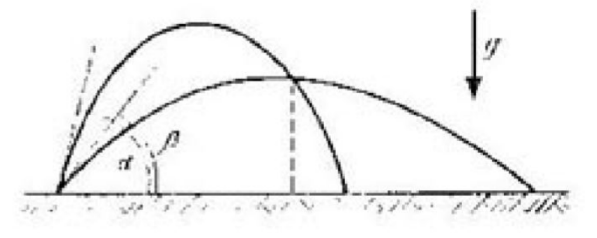
\includegraphics[scale=0.3]{./img/chorros.png}
		\end{figure}
	\end{ejercicio}
\end{mdframed}








\begin{mdframed}[style=warning]
	\begin{ejercicio}
		Una bola es lanzada hacia arriba de un plano con rapidez $v_o$. El plano esta inclinado con respecto a la horizontal un ángulo $\phi$ y la velocidad inicial de la bola forma un ángulo $\theta$ con el plano. Encuentre la distancia, medida a lo largo del plano inclinado, del punto de lanzamiento al punto donde la bola golpea el plano. Y muestre que para un $v_o$ y un $\phi$ dados, la distancia máxima de la bola es
			$$ R_{max} = \frac{v_o ^2}{g(1 + \sin{\phi})}. $$
	\end{ejercicio}
\end{mdframed}







\begin{mdframed}[style=warning]
	\begin{ejercicio}
		Una partícula se mueve horizontalmente en movimiento circular uniforme sobre un plano $xy$. En cierto instante se mueve a través del punto ordenado $(4m,4m)$ con una velocidad de $-5\vx \, m/s$ y una aceleración de $12.5\vy \, m/s^2$. ¿Cuáles son las coordenadas del centro de la trayectoria circular?
	\end{ejercicio}
\end{mdframed}










\begin{mdframed}[style=warning]
	\begin{ejercicio}
		Un tren va a $20m/s$ hacia el norte. Un niño dentro de él juega con un carrito de juguete y lo lanza sobre el piso del vagón con una rapidez de $4m/s$. Calcule cuál es la velocidad del carrito vista por un observador en la tierra, si el niño lanza el carrito:
		\begin{enumerate}[a)]
			\item En el mismo sentido de la velocidad.
			\item En sentido opuesto.
			\item Hacia el este.
		\end{enumerate}
	\end{ejercicio}
\end{mdframed}






























%%%